\section{Calculation of $R_0$ from standard
  methods}\label{app:R0_standar_methods}

The standard methods of calculation of $R_0$ are based in the linear
stability analysis of the disease-free equilibrium, either directly, through
the linear analysis of the fixed point, that yields the stability condition
from which $R_0$ can be obtained, or using the Next Generation Method (NGM)
\cite{Diekmann2010} that provides directly $R_0$ by solving a suitable linear
problem. Customarily these methods are applied to a pre-pandemic disease-free
equilibrium, but as there is no such state in the case of non-stationary
populations, here a similar approach is applied to a post-pandemic or
asymptotic disease-free equilibrium.

\subsection*{Linear stability analysis}

In order to perform the linear stability analysis of the fixed point
($I_H=I_v=0$) we first need to compute the Jacobian matrix, $J$,
\begin{equation}
    J = \begin{pmatrix}
        -\beta \frac{I_v}{N_H} & 0                       & 0       & - \beta
        \frac{S_H}{N_H}                                                      \\
        \beta  \frac{I_v}{N_H} & -\gamma                 & 0       & \beta
        \frac{S_H}{N_H}                                                      \\
        0                      & -\alpha \frac{S_v}{N_H} & -\alpha
        \frac{I_H}{N_H} - \mu  & 0                                           \\
        0                      & \alpha \frac{S_v}{N_H}  & \alpha
        \frac{I_H}{N_H}        & - \mu                                       \\
    \end{pmatrix}
\end{equation}
Then, we evaluate the Jacobian at the fixed point (or disease
free equilibrium, DFE), yielding
\begin{equation}
    J\rvert_{DFE} = \begin{pmatrix}
        0     & 0                                       & 0 & - \beta \\
        0     & -\gamma                                 & 0 & \beta   \\
        0     & -\alpha \frac{C}{N_H}\frac{\delta}{\mu} &
        - \mu & 0                                                     \\
        0     & \alpha \frac{C}{N_H}\frac{\delta}{\mu}  & 0
              & - \mu                                                 \\
    \end{pmatrix}
    \label{eq:DFEmatrix}
\end{equation}
where $S_H=N_H$ has been considered.

The eigenvalues of \cref{eq:DFEmatrix} are,
\begin{equation}
    \begin{split}
        \lambda_0 &= 0 \\
        \lambda_\mu &= -\mu \\
        \lambda_{\pm} &= -\frac{(\gamma+\mu)}{2} \pm
        \frac{1}{2}\sqrt{ (\gamma-\mu)^2 +4\beta \alpha
            \frac{C}{N_H}\frac{\delta}{\mu}
        }
    \end{split}
\end{equation}

It is straightforward to see that all eigenvalues are real and
the stability of the disease-free equilibrium is determined by the sign of the
eigenvalues. $\lambda_\mu = -\mu <0$ as $\mu$ is defined positive, so  in order
to discuss the stability of this fixed point, we need to study the
$\lambda_{\pm}$ eigenvalues. $\lambda_{-}$ is always negative, but
$\lambda_{+}$ changes sign depending on the values of the parameters. The
threshold condition $\lambda_{+} = 0$ leads to:
\begin{equation}
    \lambda_{+} = 0 \; \Rightarrow \; \frac{\beta
        \alpha}{\gamma \mu} \frac{C}{N_H}\frac{\delta}{\mu} = 1
    \label{eq:lambda+_general}
\end{equation}
So, for $\displaystyle\frac{\beta \alpha}{\gamma \mu}
    \frac{C}{N_H}\frac{\delta}{\mu}<1 \, \Rightarrow \, \lambda_{+} < 0 $ the
fixed
point is stable and for $\displaystyle\frac{\beta \alpha}{\gamma \mu}
    \frac{C}{N_H}\frac{\delta}{\mu} >1 \, \Rightarrow \, \lambda_{+} > 0 $ a
perturbation will grow in the direction of the eigenvector associated to
$\lambda_{+}$. Thus, this threshold defines the basic reproduction number,
\begin{equation}
    R_0 = \frac{\beta \alpha}{\gamma
        \mu}\frac{C}{N_H}\frac{\delta}{\mu}
\end{equation}

If instead of $S_H=N_H$ one considers any initial condition of
hosts, $S_H(0)$, the basic reproduction number is given by,
\begin{equation}
    R_0 = \frac{\beta \alpha}{\gamma
        \mu}\frac{C}{N_H}\frac{\delta}{\mu}\frac{S_H(0)}{N_H}
\end{equation}

\subsection*{Next Generation Matrix method}

The previous result can also be obtained by means of the NGM method,
which is explained in detail in\cite{Diekmann2010}. Basically the method is
based in decomposing the Jacobian in the form
$J=T+\Sigma$, where $T$ is the
\textit{transmission part}, that describes the production of new infections,
and $\Sigma$ the \textit{transition part}, that describes changes of
state (including death). Then, it can be proved \cite{Diekmann2010} that the
\textit{basic reproduction number} $R_0$ is given by the spectral radius (i.e.
the largest eigenvalue) of the (next generation) matrix $K=-T \Sigma^{-1}$.
\begin{equation}
    K=- T \Sigma^{-1} =
    \begin{pmatrix}
        \frac{\beta \alpha}{\gamma
        \mu}\frac{C}{N_H}\frac{\delta}{\mu} & \frac{\beta}{\mu} \\
        0                                   & 0                 \\
    \end{pmatrix}
    \label{eq:NGM_general}
\end{equation}
with,
\begin{equation*}
    \begin{aligned}
         & T =
        \begin{pmatrix}
            0 & \beta\frac{N_H}{N_H} \\
            0 & 0
        \end{pmatrix} \, , \qquad
        \Sigma =
        \begin{pmatrix}
            -\gamma                                & 0    \\
            \alpha \frac{C}{N_H}\frac{\delta}{\mu} & -\mu
        \end{pmatrix} \\
         & \textrm{and} \quad
        -{\Sigma}^{-1} =
        \begin{pmatrix}
            \frac{1}{\gamma}                                        & 0
            \\

            \frac{\alpha}{\gamma\mu}\frac{C}{N_H}\frac{\delta}{\mu} &
            \frac{1}{\mu}
        \end{pmatrix}
    \end{aligned}
    \label{eq:F-V_general}
\end{equation*}

The basic reproduction number is the spectral radius of this
matrix so:
\begin{equation*}
    \begin{aligned}
        det(K-\sigma\mathbb{I}) & = 0 \implies
        \begin{vmatrix}
            \frac{\beta \alpha}{\gamma
            \mu}\frac{C}{N_H}\frac{\delta}{\mu} -\sigma & \frac{\beta}{\mu } \\
            0                                           & -\sigma            \\
        \end{vmatrix} = \\
                                & = (-\sigma)\bigg(\frac{\beta
            \alpha}{\gamma
            \mu}\frac{C}{N_H}\frac{\delta}{\mu} -\sigma\bigg)  =0 \ .
    \end{aligned}
\end{equation*}

Solving for $\sigma$ one obtains the solutions,
\begin{equation}
    \sigma_1 = \frac{\beta \alpha}{\gamma
        \mu}\frac{C}{N_H}; \quad \sigma_2 = 0
\end{equation}
Therefore, the basic reproduction number is
\begin{equation}
    R_0 = \frac{\beta \alpha}{\gamma
        \mu}\frac{C}{N_H}\frac{\delta}{\mu}
\end{equation}

If instead of $S_H=N_H$ one considers any initial condition of hosts,
$S_H(0)$, the basic reproduction number is given by,
\begin{equation}
    R_0 = \frac{\beta \alpha}{\gamma
        \mu}\frac{C}{N_H}\frac{\delta}{\mu}\frac{S_H(0)}{N_H}
\end{equation}

\section{Calculation of $R_0$ for non-stationary vector populations}
\label{app:R0_non_stationary}

We extend the computation of $R_0$ in the case of non-stationary and
non-periodic vector populations by following the natural definition of
\textit{basic reproductive number}. Thus, $R_0$ is computed by averaging the
number of  secondary infections produced by an infected individual along one
generation, that is equivalent to averaging the instantaneous definition of
$R_0$, namely $R_0^i$, over one generation,
\begin{equation}\label{eq:R_eff_to_integrate}
    \overline{R_0}=\avg{R_0^i(t)}\Big\rvert\limitss{0}{t_g}=
    \frac{R_0}{N_v^*}\avg{N_v(t)}\Big\rvert\limitss{0}{t_g}=
    \frac{R_0}{N_v^*}\frac{1}{t_g}\int_0^{t_g}N_v(t)
    \, \dif t \ ,
\end{equation}
where the integral in \cref{eq:R_eff_to_integrate} is solved as
\begin{equation}
    \begin{aligned}
         & \int_0^{t_g}N_v(t) \, \dif t=\claudator{N_v^*t
        -\frac{1}{\mu}\parentesi{N_v(0)-N_v^*}e^{-\mu t}}\limitss{0}{t_g}=   \\
         & N_v^*t_g -\frac{1}{\mu}\parentesi{N_v(0)-N_v^*}\claudator{e^{-\mu
                    t_g} - 1} \ .
    \end{aligned}
\end{equation}
Thus, the basic reproduction number for non-stationary vector populations
is given by
\begin{equation}
    \overline{R_0}=\frac{R_0}{N_v^*}\left\{N_v^*-\frac{1}{\mu
        t_g}\claudator{N_v(0)-N_v^*}\claudator{e^{-\mu t_g}-1}\right\} \ ,
    \label{eq:r0mdef}
\end{equation}
where the generation time, $t_g$, is \cref{eq:generationtime}.
%    \begin{equation}
%        t_g=\frac{1}{\gamma}+\frac{1}{\mu}\ .
%        \label{eq:tgen}
%    \end{equation}
\cref{eq:r0mdef} can be rewritten as,
\begin{equation}
    \overline{R_0}=\avg{R_{0}^{i}(t)}\Big\rvert\limitss{0}{t_g}=
    R_0\claudator{1-\frac{1}{\tau}\parentesi{f-1}
        \parentesi{e^{-\tau}-1}}=R_0\cdot\mathcal{F}
    \ ,
    \label{eq:R0_non_stationary2}
\end{equation}
where $\tau=1+\mu/\gamma$ and $\mathcal{F}$ is the expression in brackets,
which accounts for the effect of the decaying vector population on the
stationary $R_0$.

In our approach, a generation is defined as the time elapsed in the
following sequence of processes: 1) A host individual becomes infected; 2) The
infected host passes the disease to a susceptible vector; 3) The infected
vector dies. Basically, the time elapsed from the first to the last process is
the time in which new infections can be produced, i.e., $t_g$
\cref{eq:generationtime}.

% \section{Vector population dynamics for Xf diseases}\label{app:vector_dynamics}

% \cref{fig:vector_dynamics} shows a time series for the population of
% \textit{Philaenus spumarius} in Mallorca, taken from \cite{Lopez2021} (in
% blue). Superimposed (in orange) is the assumption used in our model
% \cref{eq:SEIR_v}, the $\delta(t-nT)$, i.e., every year susceptible vectors
% appear in the system.

% \begin{figure}
%     \centering
%     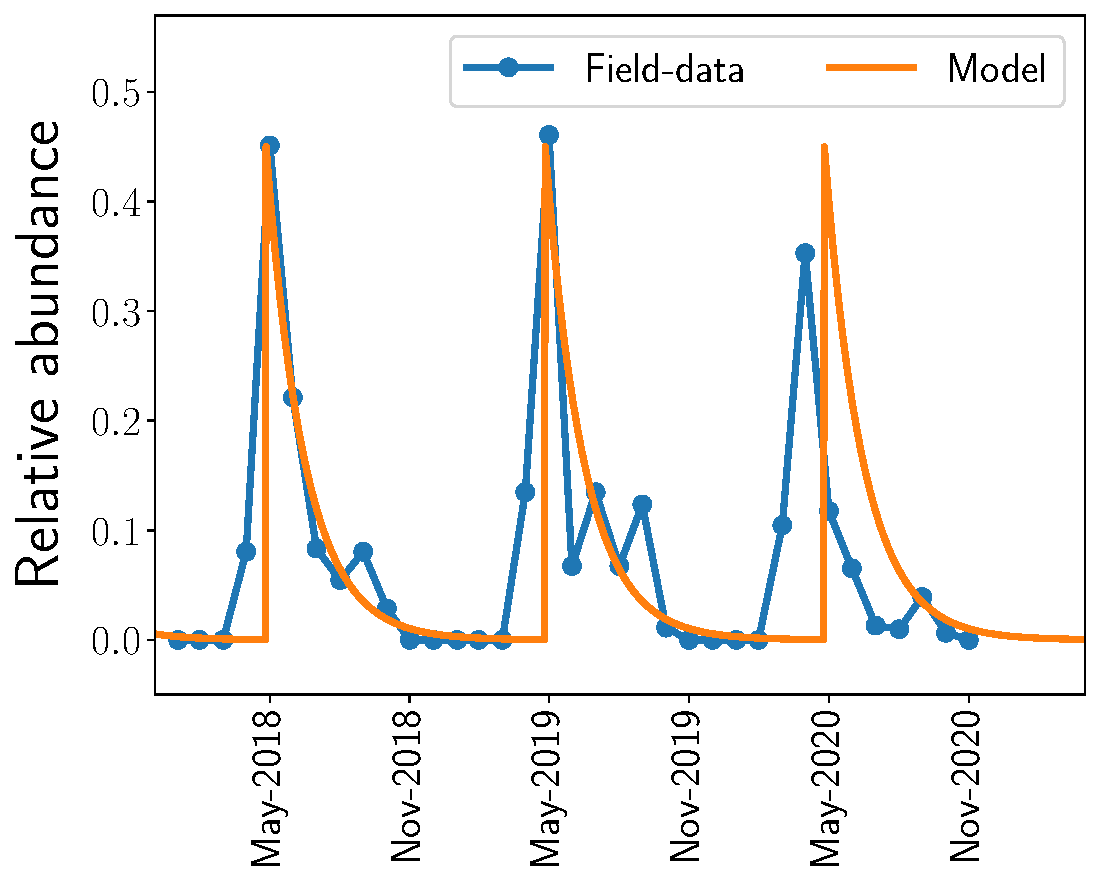
\includegraphics[width=0.7\textwidth]{Figures/Vector_dynamics.pdf}
%     \caption[Vector dynamics produced by the model compared to
%         field-data]{Vector dynamics produced by the model compared to
%         field-data
%         from \cite{Lopez2021}.}
%     \label{fig:vector_dynamics}
% \end{figure}

\section{Determination of $R_0$ for Xf diseases}\label{app:R0}

The handicap of determining the basic reproductive number of the model
\cref{eq:SEIR_v} is that the pre-pandemic fixed point given by $I_H=I_v=0$ and
$S_H=S_H(0)$ is not a fixed point of the system of differential equations,
because vector population decays, so that the standard methods to compute $R_0$
such as the Next Generation Matrix \cite{Diekmann2010, GimenezRomero2022_PRE}
do not
apply. In \cite{GimenezRomero2022_PRE} a method was suggested to determine
the basic
reproductive number in the case of compartmental models of vector-borne
transmitted diseases in which the vector population grows or decays. It
consists in averaging the instantaneous basic reproductive number over the time
of a generation.

To proceed we consider that $I_H=I_v=0$, $S_H=S_H(0)$ is indeed a fixed
point of the system. Then, the basic reproductive number could be determined,
e.g., as shown in \cite{Brauer2016}. First, an infectious host infects vectors
at a rate $\beta S_H(0)/N_H$ for a time $1/\gamma$. This produces $\beta
    S_H(0)/\gamma N_H$ infected vectors. The second stage is that these
infectious
vectors infect hosts at a rate $\alpha N_v(0)/N_H$ for a time $1/\mu$,
producing $\alpha N_v/\mu N_H$ infectious hosts per vector. The net result of
these two stages is
\begin{equation}
    \tilde{R}_0=\frac{\alpha\beta}{\mu\gamma}
    \frac{S_H(0)}{N_H^2}N_v(0)=R_0^*
    \cdot
    N_v(0)\ .
    \label{eq:R0tilde}
\end{equation}
This result coincides with the value of $R_0$ obtained using the standard
NGM method, that can be applied in this case because we are assuming that we
use a nongeneric initial condition that sits at the fixed point of the model.

In practice, our initial condition will never be a fixed point of the
model, and, as mentioned above, we will obtain an approximate basic
reproductive number, to which we will refer as $R_0$ using the method suggested
in \cite{GimenezRomero2022_PRE}, that consists in
%\cite{Gimenez2022}). 
calculating the \textit{average} number of secondary infections produced by
an infectious host in \textit{one generation}. One first defines an
instantaneous basic reproductive number,
\begin{equation}\label{eq:R0i}
    R_0^{(i)}(t)=\frac{\beta\alpha}{\mu\gamma}\frac{S_H(0)}{{N_H}^2}
    N_v(t)=R_0^* N_v(t) \ ,
\end{equation}
from which the average is simply computed as
\begin{equation}\label{eq:R_eff_to_integrate}
    R_0=\avg{R_0^{(i)}(t)}\Big\rvert\limitss{0}{\tau}=
    R_0^*\avg{N_v(t)}\Big\rvert\limitss{0}{\tau}=
    R_0^*\frac{1}{\tau}\int_0^{\tau}N_v(t)
    \, \dif t \ .
\end{equation}
In our model, the time-dependent vector population can be obtained from
\cref{eq:SEIR_v},
\begin{equation}
    \dot{N}_v=\dot{S}_v+\dot{I}_v=-\mu N_v \Longrightarrow
    N_v(t)=N_v(0)e^{-\mu t} \ ,
\end{equation}
and introducing this expression for $N_v(t)$ in
\cref{eq:R_eff_to_integrate} the integral can be solved
\begin{equation}
    R_0={{\beta\alpha S_H(0)}\over{\mu\gamma N_H ^2}}
    \,\frac{N_v(0)}{\mu\tau}\left(1-e^{-\mu\tau}\right)=
    R_0^*\ \frac{N_v(0)}{\mu\tau}\left(1-e^{-\mu\tau}\right) ,
    \label{eq:r0mdef}
\end{equation}
that is an approximated expression to the basic reproductive number for our
model, in which the vector population is nonstationary,
where, in \cref{eq:R0i} and \cref{eq:r0mdef} it has been defined, $R_0^*=
    (\beta\alpha S_H(0))/(\mu\gamma N_H ^2)$.

Note that in our model one generation correspond to one year and that
$N_v(0)$ is reset every year.